\documentclass[conference]{IEEEtran}
\IEEEoverridecommandlockouts
\usepackage[ngerman]{babel}
% The preceding line is only needed to identify funding in the first footnote. If that is unneeded, please comment it out.
\usepackage{cite}
\usepackage{amsmath,amssymb,amsfonts}
\usepackage{algorithmic}
\usepackage{graphicx}
\usepackage{textcomp}
\usepackage{xcolor}
\usepackage{setspace}
\usepackage{booktabs}
\usepackage[export]{adjustbox}
\def\BibTeX{{\rm B\kern-.05em{\sc i\kern-.025em b}\kern-.08em
    T\kern-.1667em\lower.7ex\hbox{E}\kern-.125emX}}
\begin{document}

\title{Currency Exchange, eine App zur Anzeige von Wechselkursen mit Hilfe eines Webscrapers}


\author{\IEEEauthorblockN{1\textsuperscript{st} Matz, Annika}
\IEEEauthorblockA{\textit{dept. name of organization (of Aff.)} \\
\textit{name of organization (of Aff.)}\\
Berlin, Deutschland \\
s\_matz22@stud.hwr-berlin.de}
\and
\IEEEauthorblockN{2\textsuperscript{nd} Liebenberg, Benjamin}
\IEEEauthorblockA{\textit{dept. name of organization (of Aff.)} \\
\textit{name of organization (of Aff.)}\\
Oranienburg, Deutschland \\
s\_liebenberg22@stud.hwr-berlin.de}
\and
\IEEEauthorblockN{3\textsuperscript{rd} Reetz, Tobias}
\IEEEauthorblockA{\textit{dept. name of organization (of Aff.)} \\
\textit{name of organization (of Aff.)}\\
Berlin, Deutschland \\
s\_reetz22@stud.hwr-berlin.de}
%Beispiel wie es aussah
%\and
%\IEEEauthorblockN{3\textsuperscript{rd} Given Name Surname}
%\IEEEauthorblockA{\textit{dept. name of organization (of Aff.)} \\
%	\textit{name of organization (of Aff.)}\\
%	City, Country \\
%	email address or ORCID}
}

\maketitle


\section{Einführung}
Innerhalb unseres dualen Studiums der Informatik an der "Hochschule für Wirtschaft und Recht", nahmen wir an dem Modul Software-Engineering 2 teil. Ziel dieses ist die Entwicklung von Software, vermittelt zu bekommen und das erlernte Wissen direkt anwenden zu können innerhalb einer Projektarbeit. Dabei wird auf die Grundlagen des Projektmanagments geachtet, wofür z.B. UML-Diagrammen angefertigt werden. Zur Dokumentation des Projektes wird dieses Paper angefertigt. 
Innerhalb des Moduls werden auch Softskills gefördert, z.B. die Präsentationsfähigkeiten oder die Sozialkompetenz innerhalb von Gruppenarbeiten.

\section{Idee des Projektes}
Ein sehr großer Teil unseres Lebens dreht sich um das erwerben von unterschiedlichen Materiellen Gütern. Für unserer Arbeit werden wir vergütet, im Supermarkt kaufen wir davon unser Abendessen und an den Wochenenden und im Urlaub gehen wir auf Reisen. Auf diesen müssen wir uns in einer fremden Kultur zu Recht finden und konsumieren weiter Güter. Doch wie können wir einen Wert von diesen einschätzen, wenn wir die Währung nicht kennen? Und genau dieses Problem löst unsere App "Currency Exchange". Einfaches nachschlagen von tagesaktuellen Wechselkursen und umrechnen zwischen verschiedenen Währungen. Ein besonderes Feature ist das Umwandeln des eingegebenen Wertes in die Anzahl von Döner, welche damit gekauft werden könnten in Euro. \\
Die  Android-App arbeitet mit Hilfe eines Webscrapers, welcher Wechselkurse erhält.
% und Beträge der unterschied- lichen Währungen ineinander umrechnet.

\section{Projektorganisation}
Innerhalb eines Softwareentwicklungsprojekts erhalten die einzelnen Bearbeitenden verschiedene Rollen, die ihnen unterschiedliche Aufgaben zu teilen. In diesem Fall bestand das Entwicklungsteam aus wenigen Personen, so wurden keine expliziten Arbeitsbereiche vergeben.  So wurden Aufgaben nach und nach vergeben, wobei jeder Bereich eine eigene Ansprechperson besaß. Unterteilt wurde in Projektleitung, Serveradministration, Design und Testdurchführung. Zu Anfang wurde für essentiell wichtige Themen, wie z.B. die Software-Architektur oder den groben Design-Entwurf, wurden Teammeetings durchgeführt und die Umsetzung so zusammen geplant. Sichergestellt wurde so, dass jedes Teammitglied mit einbezogen wird und alle auf dem gleichen Stand sind. \\
Die Programmierung der Software wurde von Teammeeting zu Teammeeting aufgeteilt. Hauptsächlich kümmerten sich Benjamin und Tobias Reetz um die Programmierung des Webscrapers, sowie die Schnittstelle und ein Teil des Backend der App. Annika Matz kümmert sich vor allem um die Umsetzung des Designentwurfs zu einem funktionierenden Frontend, sowie ein Teil der Programmierung des Backend.

\subsection{Projektleitung}
Der Projektleitung wurde von Annika Matz übernommen. Unteranderem behielt sie die unterschiedlichen Abgabetermine im Blick. Außerdem sorgte sie für regelmäßig Treffen in der Gruppe und leitete diese an. Bei diesen wurde der aktuelle Stand ausgewertet, weitere Entwicklungsschritte besprochen und Aufgaben verteilt. \\
Des weiteren achtete sie auch auf die Projektanforderungen und führte die Qualitätssicherung durch, wodurch sie für eine angemessene Feedback innerhalb der Teammeetings sorgt.

\subsection{Serveradministration}
Der Bereich Serveradministration wurde von Benjamin Liebenberg beaufsichtigt. Aufgrund seiner weitreichenden Erfahrung in diesem Gebiet, konnte er diesen Bereich übernehmen. Er hostet unseren Webscraper auf seinem Server, sorgt für täglich aktualisierte Daten innerhalb der App und stellt die Schnittstelle für unsere App bereit.

\subsection{Design \& Testplanung}
Das Design und die Testplanung wurden zum größten Teil von Tobias Reetz übernommen. Aufgrund seiner Designerfahrung im Modul Software-Engineering 1, übernahm er diese Rolle und designte vor allem das App-Logo. Er sorgte für eine angemessene Farbgebung und dafür, dass die App aufgrund ihrer Gestaltung schnell wieder erkennt werden kann. \\
Außerdem übernahm er das Konkretisieren von Usability-Tests, welche wir zuvor im Plemnum entworfen hatte und führte diese mit unseren Kommilitonen durch. Damit trug er einen entscheidenen Beitrag zur Fehlersuche und somit zur Qualität unseres Programmes bei.

\section{Anforderungen}
An eine Software werden immer unterschiedliche Erwartungen und Anforderungen gestellt. Eine genaue Definition sind wichtig für den Erfolg des Projektes. In diesem Projekt werden die unterschiedlichen Anforderung in drei Kategorien unterteilt. Sie beinhalten nicht funktionale, funktionale und optionale funktionale Anforderungen.

\subsection{Nicht funktionale Anforderungen}
Nicht-funktionale Tests decken alle Anforderungen ab, welche das gesamte System ansich betreffen. Es werden somit keine Funktionen abgeprüft, sondern Eigenschaften und Bestandteile. Für das Projekt wurde besonders auf eine sehr gute Usability geachtet, was besonders durch eine intuitive und einfache Benutzung begründet werden soll.
Desweiteren soll eine Verfügbarkeit des Projekt auf Android-Handys garantiert werden. Um einen hohen Datenschutz garantieren zu können erheben wir keine Daten und speichern auch nicht die in der Vergangenheit getätigten Eingaben dem Nutzer zur Verfügung. 

\subsection{Funktionale Anforderungen}
Funktionale Anforderung definieren die Funktionen und Erwartungen der Software, welche für ein erfolgreiches Projekt erfüllt werden müssen. \\
Das wichtigste Ziel für die Software ist eine lauffähige Android-Handy-Applikation, welche verschiedene Eingaben zwischen verschiedenen Währungen richtig Umrechnen kann. Es soll immer ein tagesaktueller Wechselkurs bereit stehen. In die App sollen auch mindestens sieben Währungen eingebunden werden.

\subsection{Optionale funktionale Anforderungen}
Anforderungen, welche nicht essentiell notwendig für die grundlegenden Funktionsweise sind, aber sie diese erweitern, werden zu den optionalen funktionalen Anforderungen gezählt. \\
Zu diesen zählt die Umrechnung der Anzahl an Döner, die die Nutzenden sich mit dem eingetragenen Wert kaufen könnten in Euro. Außerdem könnte die App durch eine Funktion zum Hinzufügen von Prozentualen Werten ergänzt werden. Diese könnten zum Beispiel zur Berechnung der Mehrwertsteuer oder des Trinkgeldes genutzt werden.

\section{Entwurf}
Innerhalb eines Entwurfs wird der Aufbau und die Struktur des Projektes geplant und fest gehalten. Dieser besteht in diesem Projekt aus zwei der Systemarchitektur, einem Sequenzdiagramm und dem groben Designentwurf. Nach diesen Vorgaben wurde die App entwickelt.

\subsection{Systemarchitektur}
Eine Systemarchitektur beschreibt die Struktur des Projektes, so wie alle seine vorkommenden Bereiche und wie diese miteinander interagieren. 

\begin{figure}[h]
	\centering
	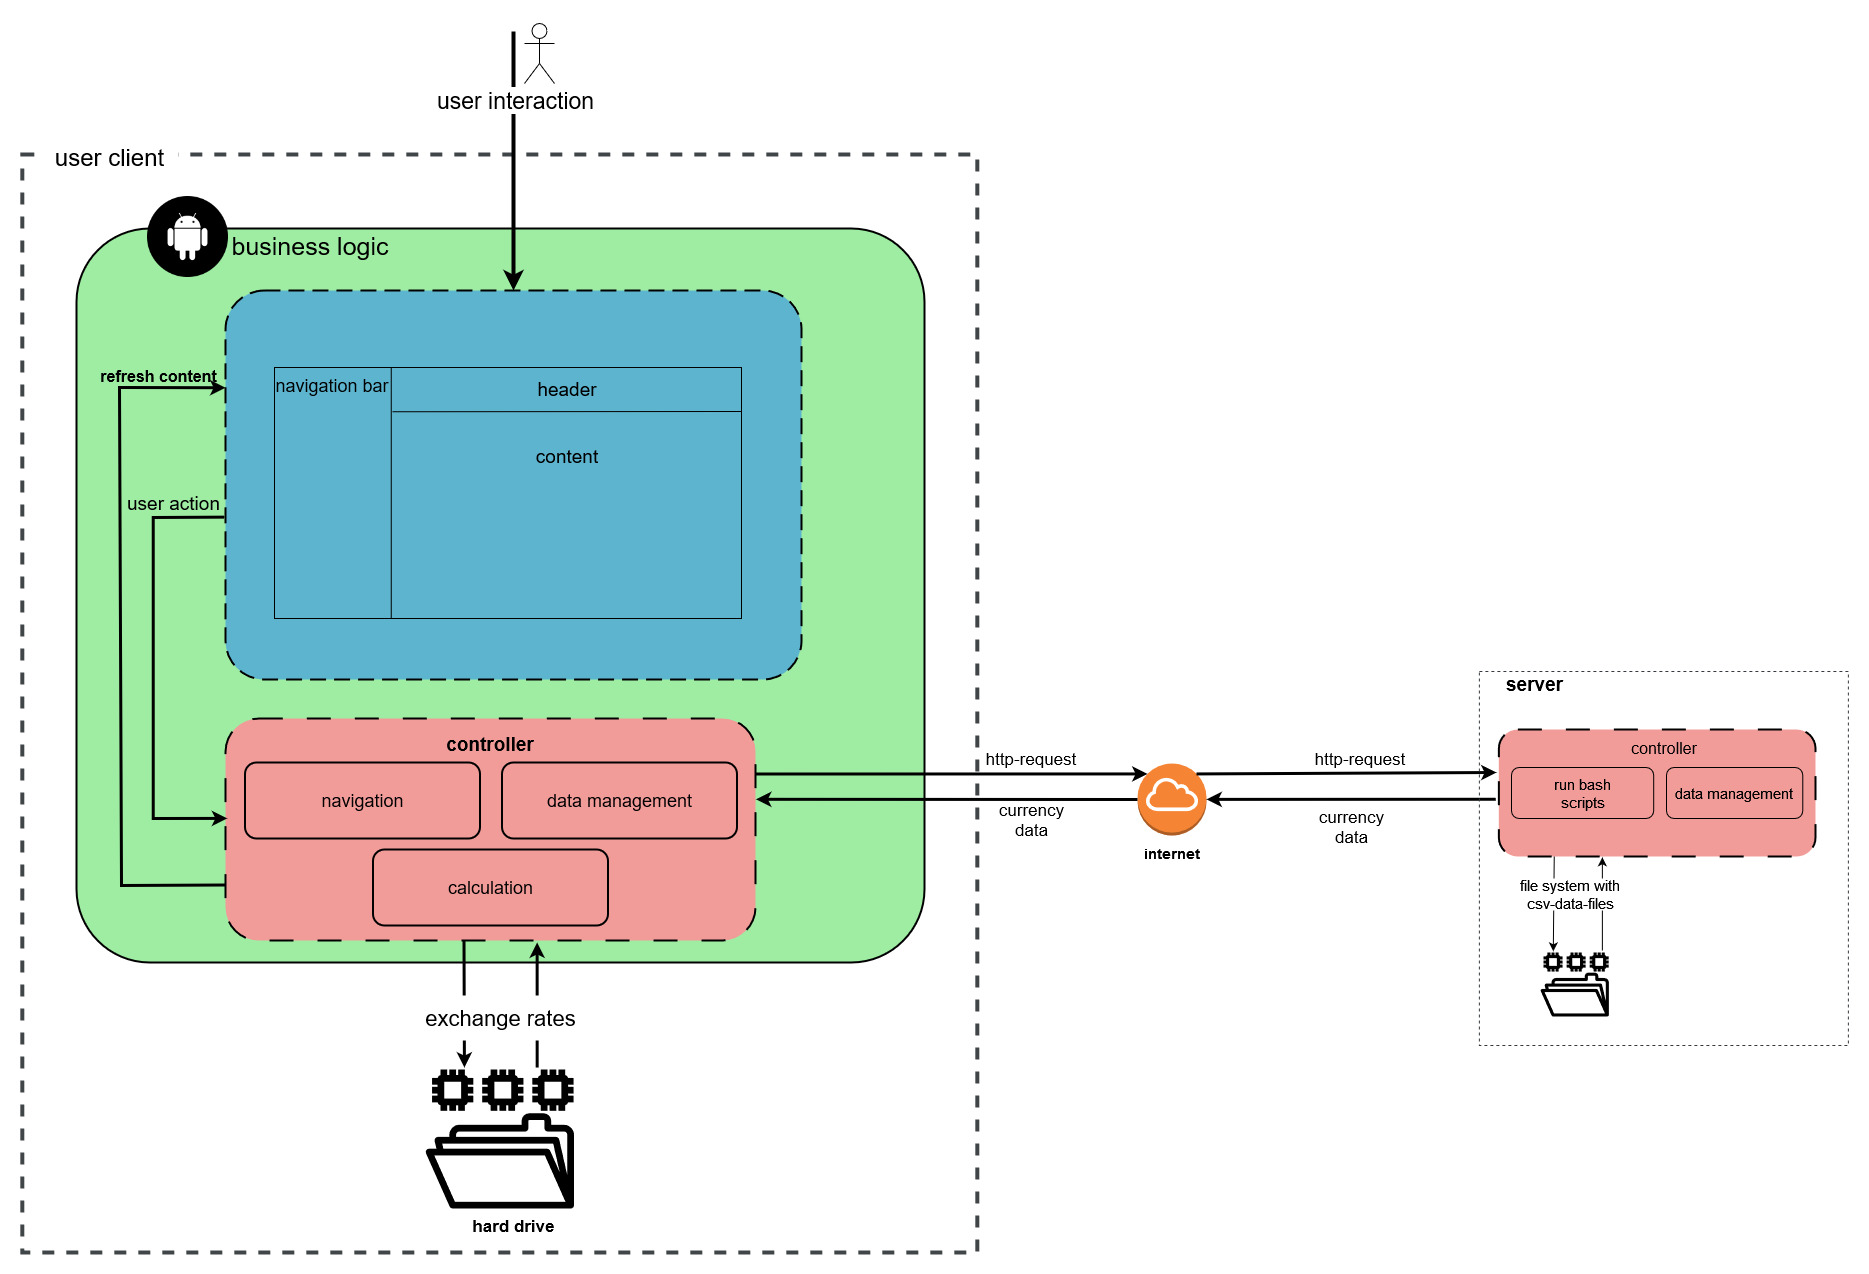
\includegraphics[width=1\linewidth, frame]{Software-Architektur_SWEII}
	\caption[Softwarearchitektur]{Softwarearchitektur}
	\label{fig:software-architektursweii}
\end{figure}
\noindent
Abbildung \ref{fig:software-architektursweii} zeigt wie die Softwarearchitektur strukturiert ist. Auf der linken Seite ist der User-Client abgebildet und auf der Rechten der Server. Aufgrund dieser zwei Komponenten, handelt es sich um eine Zwei-Tier-Architektur. \\
Im User-Client ist zusehen, dass der User mit der in blau gekennzeichneten Benutzeroberfläche interagiert. Diese besteht aus einem Header, einer Navigationsleiste, und dem Inhalt. Über die Interaktion können Nutzende verschiedene Funktionen erreichen, diese sind als Controller im roten Bereich zu sehen sind. Diese werden in drei unterschiedliche Bereiche kategorisieren, dem Navigator, der Data-Manager und der Calculator. Der Data-Manager ist dafür zuständig die Daten in einem Ordner zu speichern und sie den Anderen Funktionen bereit zu stellen. Er stellt auch Anfragen per HTTP-Request an den Server und sorgt somit für eine aktuelle CSV-Datei mit den benötigten Wechselkursen. Der Calculator berechnet die Wechselkurse und der Navigator sortiert Daten und stellt sie der Benutzeroberfläche bereit. \\
 Der Controller des Servers stellt Bash-Skripte bereit, die den Webscraper täglich starten. Der Data-Manager ist hier auch wieder für die Aufarbeitung der Daten zuständig. Dabei sorgt er für die korrekte Speicherung in eine CSV-Datei.\\
Durch die Einbindung des Webscraper auf einem externen Server, wird eine geringe Anfrage auf die Website mit den Wechselkursen garantiert. Denn sollten zu viele Anfragen an die Webseite geschickt werden, kann es zu einer Überlastung dieser kommen. Mögliche folgen wären das Abstürzen dieser Seite.

\subsection{Sequenzdiagramm}
Das Sequenzdiagramm beschreibt die Kommunikation der unterschiedlichen Instanzen miteinander innerhalb der Software. 

\begin{figure}[h]
	\centering
	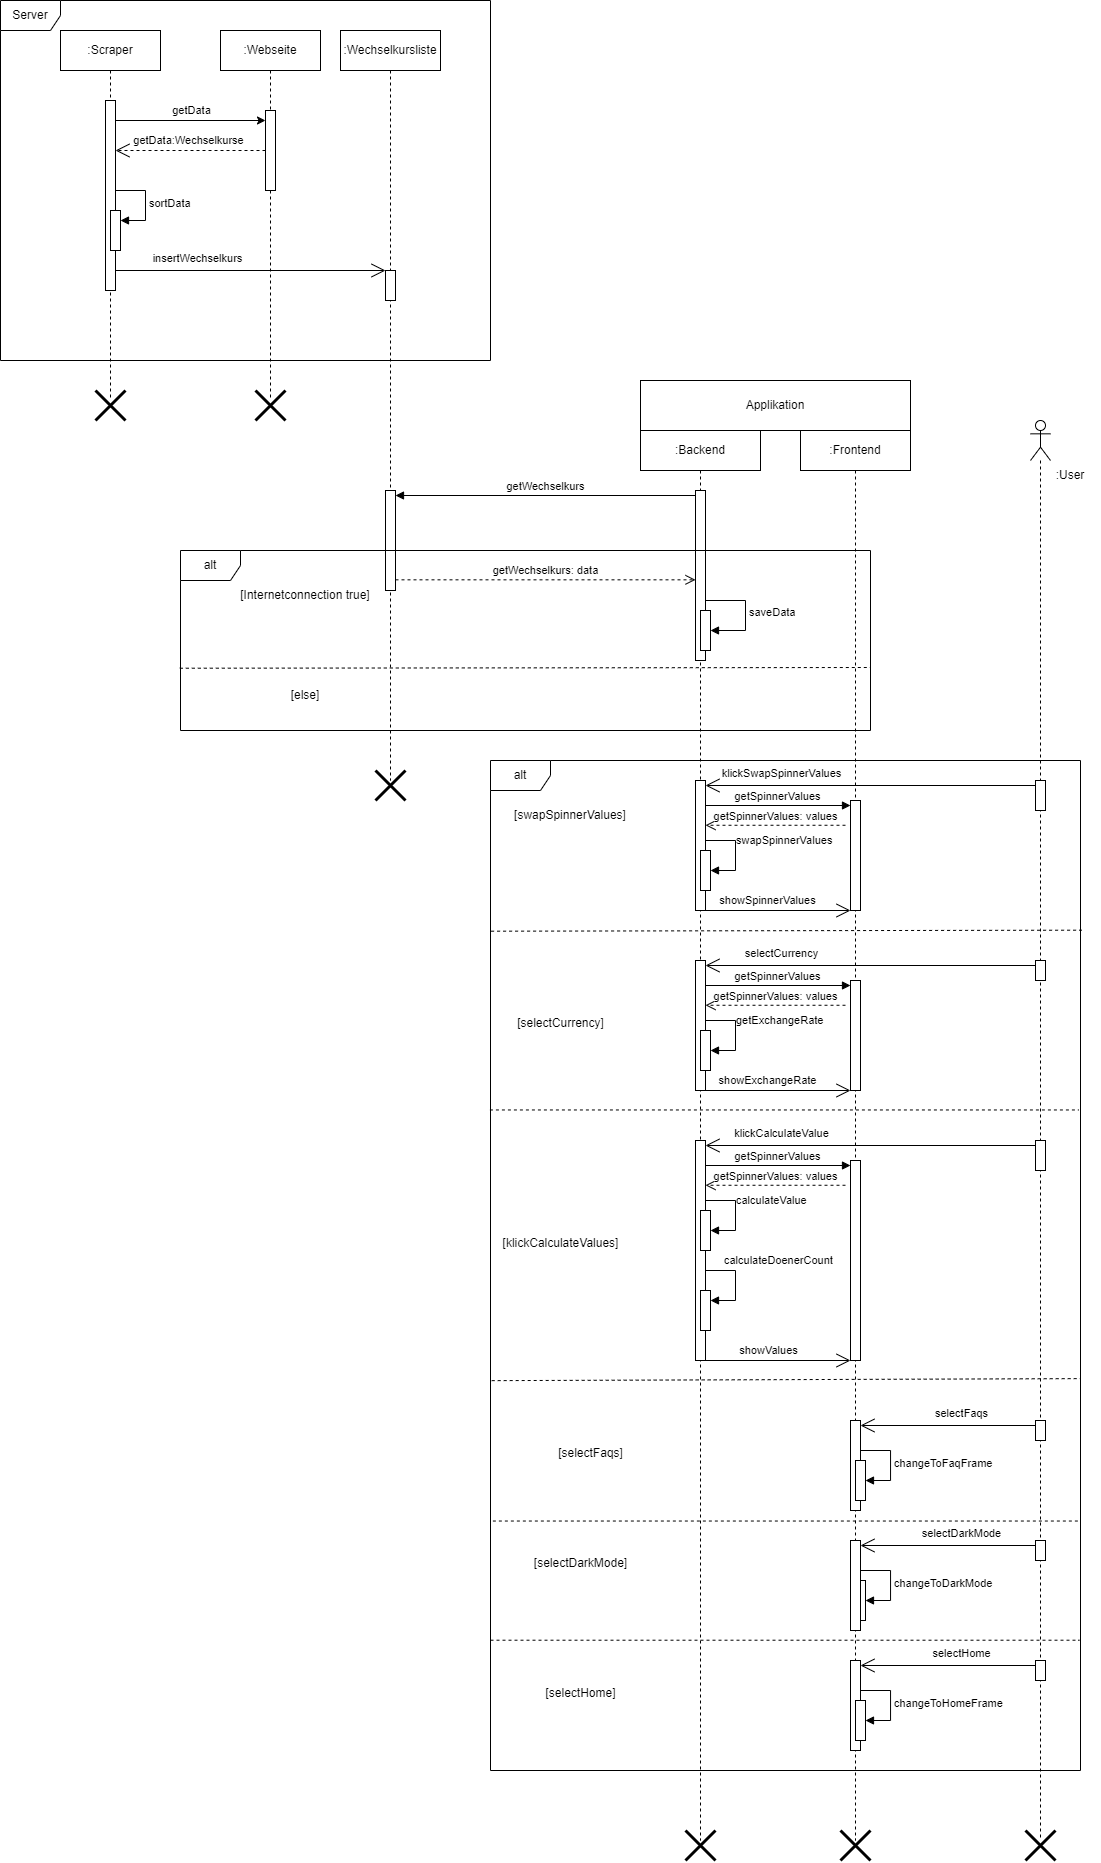
\includegraphics[width=1\linewidth, frame]{Sequenzdiagramm.drawio}
	\caption[Sequenzdiagramm]{Sequenzdiagramm}
	\label{fig:sequenzdiagramm}
\end{figure}

\noindent
Abbildung \ref{fig:sequenzdiagramm} zeigt die Gestaltung des Projektes auf. Oben links ist der Serverbereich abgebildet. Dabei holt sich der Webscraper die Daten von einer fest definierten Webseite. Danach werden diese strukturiert, alphabetisch sortiert und dann in einer CSV-Datei gespeichert. Nachfolgend ist die Applikation dargestellt. Diese ist in ein Front und Backend eingeteilt. \\
Das Backend schickt eine Anfrage an den Server um die aktuelle CSV-Datei zu erhalten. Jedoch nur wenn eine Verbindung zum Internet existiert, erhält er diese auch und kann sie speichern. Sollte keine Verbindung aufgebaut werden können, so wir die zu letzt aktualisierte CSV-Datei genutzt. \\
Innerhalb der Applikation kann der User unterschiedliche Funktionen auswählen. Die ersten drei abgebildeten Optionen haben eine ähnliche Struktur. Die nutzende Person schickt eine Anfrage an das Backend. Dieses holt sich dann die eingegebenen Daten aus dem Frontend. Wenn nun die Werte getauscht werden sollen, tauscht das Backend die Werte und übermittelt die neun dem Frontend. Wird jedoch stattdessen eine neue Währung gewählt, so wird der neue Wechselkurs im Backend berechnet und anschließend im Frontend verändert. Soll eine Umrechnung stattfinden wird zuerst der Betrag in die ausgewählte Währung übergeben und nachfolgend die Anzahl der Döner berechnet. Auch diese neuen Werte werden dann über das Frontend dem Nutzer angezeigt. \\
Zum Wechseln der Seite auf die Home-Seite bzw. der FAQ-Seite und zum Wechseln in den Dark-Mode bzw. Light-Mode navigiert der User sich durchs Frontend.

\section{Implementierung}

\subsection{Konsistenz}

\subsection{Vorbereitung}
Innerhalb der Vorbereitungsphase werden wichtige Punkte für den Verlauf des Projekts festgelegt. Einer dieser Punkte ist die Versionsverwaltung. Über sie werden die verschiedenen Stände der Software gesteuert und überblickt. Außerdem kann im Fall von irreversiblen Fehlern auf frühere Versionen zugegriffen werden, wodurch es vermieden wird händisch den gesamten Code auf einen früheren Stand um zu strukturieren, was bei großen Codemengen sehr zeitaufwändig ist und somit viel Zeit der Bearbeitung einspart. Dazu wurde die Plattform GitHub verwendet, weil sie verständlich gestaltet worden ist und somit wenig Zeit für die Einarbeitung benötigt. Zu dem ist GitHub kostenfrei und weit verbreitet, was bei Problemen mit der Versionsverwaltung zu einem breiten Angebot von Hilfestellungen führt, da wahrscheinlich das Problem schon irgendwann mal aufgetaucht ist.\\
Ein weiterer Punkt ist die Namenskonvention von Funktionen, Variablen und Dateien. Hierbei wurde festgelegt, dass die Namen deskriptiv sein sollen, damit sie möglichst einfach zu verstehen sind. Deskriptive Namen werden so gestalten, dass der Namen alleine die Funktionalität beschreiben kann, wodurch auch viele Kommentarzeilen eingespart werden können, weil der Name diese Funktion schon übernimmt und eine genauere Beschreibung selten benötigt wird.\\
Der wichtigste Punkte innerhalb eines Softwareprojekts sind die verwendete Entwicklungsumgebung und verwendeten Programmiersprachen. Da das Ziel bei Currency Exchange durch eine Android-App dargestellt wird, wurde nach einer Entwicklungsumgebung gesucht, die den Entwicklungsprozess durch Verbesserungsvorschläge und graphische Darstellungen der Applikation unterstützt. Eine solche Entwicklungsumgebung ist Android-Studio verwendet, weil sie ohne weitere Einstellungen Codeverbesserungen vorschlägt und einen eingebauten Emulator besitzt, der es vereinfacht die Anwendung graphisch wahrzunehmen, zu simulieren und Fehler während der Laufzeit zu finden. Dies wird des Weiteren auch durch die Namensgebung unterstrichen. Innerhalb von Android-Studio besteht die Möglichkeit zwischen den zwei Programmiersprachen Kotlin und Java zu wählen, welche beide Objekt orientierte Sprachen sind. Durch die bereits vorhandenen Vorkenntnisse des Projektteams mit der Programmiersprache Java, wurde sie als Entwicklungssprache ausgewählt, weil somit die Einarbeitungszeit in eine neue Sprache eingespart werden konnte und direkt mit der Entwicklung der Applikation begonnen werden konnte.

\section{Integration}
Die Integration in der Softwareentwicklung beschäftigt sich mit den Schnittstellen zwischen den unterschiedlichen Systemkomponenten und der Testung dieser, da es wichtig ist, dass diese miteinander kompatibel sind und bei den Übertragungen der zwischen Komponenten keine Fehler auftreten. Hierzu stehen den entwickelnden Personen diverse Methoden zur Verfügung, von denen eine die Top-Down Integration ist, welche sich dadurch kennzeichnet, das obere Schichten zu erst integriert und die unteren Schichten durch Simulationen dargestellt werden, wodurch die Grundfunktionalitäten erst einmal getestet und validiert werden können, bevor dann im darauffolgenden Schritt die Komponenten zusammengeführt und erneut überprüft werden.\\
Im Fall von Currency Exchange bedeutete dies, dass im ersten Schritt der User-Client, welcher mit Hilfe von fest eingebauten Werten getestet wurde, und der Webscraper, der die CSV-Datei über einen Port zugänglich macht und überprüft wurde, ob alle Daten richtig sortiert wurden, integriert. Im zweiten Schritt wurde die beiden Komponenten zusammen geführt und bildeten ein neues System, welches dann erneut überarbeitet und getestet worden ist. 

\section{Tests}
Um zu validieren, dass die Software in ihren Funktionen korrekt ist, muss diese ausreichend getestet werden. Dazu müssen die Funktionen, die Persistenz und die Handhabung überprüft werden. Um dies zu bewerkstelligen, wird von Testmethoden Gebrauch gemacht. Da es jedoch kaum möglich ist, alle Bestandteile der Software gleichzeitig zu testen, wird die Überprüfung in mehrere Schichten unterteilt.\\
Vor allem während der Implementierungsphase, also der eigentlichen Entwicklung der Applikation, wird hierzu auf das Experience-based Testing zurückgegriffen. Dabei werden die geplanten Funktionen standardmäßig implementiert und anschließend auf Korrektheit getestet. Vorteil dieser Testmethode ist es, dass die Funktionen und Hintergrundprozesse bekannt sind. Somit kann der Entwickler Fehler direkt ausfindig machen und möglichst unmittelbar an der Behebung dieser arbeiten.\\
Jedoch birgt diese Testmethode auch Risiken. Schließlich kann es vorkommen, dass Fehler in früheren Implementierungen entstehen, die womöglich beim Testen der neuen Funktionalitäten nicht auffallen. Aus diesem Grund wurde während der Erstellung der Software zusätzlich auf das sogenannte Beta-Testing zurückgegriffen. Dabei wird die Software von Personen getestet, welche mit den Funktionen und der Benutzeroberfläche nicht vertraut sind. Dadurch kann es zu einer Fehlbedienung kommen, welche aus Sicht der Entwickler:innen im schlechtesten Falle zu einem Absturz des Programms führt, im besten Fall nur einen Fehler auswirft. Außerdem füllen die Personen nach dem Testen der Applikation einen kurzen Fragebogen aus, welcher vor allem die Dokumentation der Fehler und Anregungen für etwaige Verbesserungen zum Thema hat. Sinngemäß beinhaltet das Beta-Testing also die Testmethoden für die Benutzerfreundlichkeit (eng. usability-tests), als auch für die Funktionalitäts-Tests (Black-Box-Testing).
Mit diesen gewonnen Daten kann die Anwendung anschließend verbessert  und mögliche Fehler beseitigt werden. \\
Im Fall von Currency Exchange wurde ein Beta-Test am 13.03.2024 durchgeführt, welcher aufschlussreiche Informationen über die Verbesserung der Applikation geliefert hat. Beispielsweise wurden einige Fehler gefunden, die den Absturz der Software zur Folge hatten. Außerdem wurden Anregungen hinsichtlich der Benutzeroberfläche und Bedienung getätigt, welche eine Überarbeitung des Designs zur Folge hatten.

\section{Wartung}

\section{Rollout}

\section{Ergebnis}

Die entwickle Software läuft komplikationslos und erfüllt alle Grundanforderungen, sowie vereinzelt optionale funktionale Anforderungen. Darunter fällt die Berechnung in Döner.  Das Abziehen bzw. Hinzufügen von prozentualen Anteilen konnte bedauerlicherweise nicht umgesetzt werden. Die Grundanforderung, dass min. 7 Währungen angeboten werden konnten wir bei weitem übertreffen.\\
Herausforderungen brachte vor allem das Design des Frontends der App. Innerhalb der Implementierung stellten wir fest, dass einige Funktionen fehlen oder aber auch zu viel sind. So kam über die weitere Entwicklung der App eine textliche Anzeige der umgerechneten Werte hinzu. Diese soll die Bedeutung der einzelnen Werte verdeutlichen und für eine bessere Verständlichkeit sorgen. Leider wurde aufgrund dieser Zustände die Benutzeroberfläche sehr voll, wodurch der Button mit dem Fragezeichen entfernt werden musste. Wir entschieden uns für dieses Element, da der Button nur eine Ergänzung zum Hamburger-Menü und der dortigen Seitennavigation gewesen ist. Von diesem wäre der Nutzer auch nur zur Informationsseite gekommen. \\
Verbessert werden könnte noch die Auswahl der Währung innerhalb der Spinner. Aufgrund einer einfachen Umsetzung konnten sehr viele Währungen angeboten werden. Dies führt leider jedoch zu einer sehr unübersichtlichen Liste, welche sehr lang ist. Zur Lösung könnte eine Suchfunktion implementiert werden, welche die begehrte Währung herausfiltert. Durch diese Erfahrungen konnte die Gruppe ihre Kompetenzen in der Front-End Entwicklung weiter aus bauen, welche zuvor nur bedingt vorhanden war.

\section{Abschluss}
Insgesamt konnte das Projekt erfolgreich abgeschlossen werden. Die Fähigkeiten innerhalb der Software Entwicklung konnten weiter vertieft und ausgebaut werden, sowie eine lauffähige Software entwickelt und alle erforderlichen Abgaben konnten getätigt werden.
Besonders gut verlief die Arbeit innerhalb der Teammeetings. Es war dauerhaft eine konstruktive Arbeitsatmosphäre, in welcher vor allem in der Phase der Konzeptionierung zielgerichtet diskutiert werden konnte. Auch während des Debuggens in der Gruppe konnte gemeinsam schnell fehlerhafter Code korrigiert werden. So konnten wir schnelle Ergebnis erreichen. \\
Vereinzelt traten Schwierigkeiten in der Kommunikation während der Implementierung auf. So entstanden Situationen, bei welchen die Gruppenmitglieder sich falsch verstanden oder nicht alle wichtigen Informationen zwischen ihnen transferiert werden konnten. Dies konnte jedoch durch die vielen Gruppenmeetings und Absprachen schnell behoben bzw. korrigiert werden, sodass sie zu keinem größeren Problem innerhalb der Gruppe führen konnten. Durch diese Erfahrungen konnten wir unsere Softskills innerhalb der Kommunikation untereinander verbessern.


\end{document}
